\documentclass[10pt,a4paper]{article}
\usepackage[latin1]{inputenc}
\usepackage{amsmath}
\usepackage{amsfonts}
\usepackage{amssymb}
\usepackage{graphicx}
\usepackage{amsthm}
\graphicspath{{images/}}

\newcommand{\R}{\mathbb{R}}

\begin{document}

\theoremstyle{definition}
\newtheorem{defn}{Definition}[section]


	\section{Basic definitions}

	\begin{defn}{\textbf{Support}}
		The set of values a random variable can take (set of all the numerical realizations of outcomes) e.g. for a binary random variable X, it's support is $R_X = \{ 0, 1 \}$
	\end{defn}


	\begin{defn}{\textbf{Sample Point}}
		In an experiment, a sample point is one of the possible outcomes of experiment denoted by $\omega$
	\end{defn}

	\begin{defn}{\textbf{Independent Events}}
	Two events A and B are independent if and only if \\
	\begin{align}
		P(A \cap B) = P(A) * P(B)
	\end{align}
	\end{defn}

	\begin{defn}{\textbf{Jointly/Mutually Independent Events}}
	Let $E_1, ... , E_n$ be n events. \\
	$E_1, ... , E_n$ are jointly independent(or mutually independent)
	if and only if for any sub-collection of k events $(k \leq n) E_{i1}, ... , E_{ik}$:
	\begin{align}
	P(\bigcap \limits_{j=1}^kE_{ij}) = \prod_{j=1}^{k}P(E_{ij})
	\end{align}
	\end{defn}

	\begin{defn}{\textbf{Random Variable}}
		A random Variable $X$ is a function from sample space $\Omega$ to set of real numbers $\R$, i.e $ X: \Omega -> \R $.\\
		
		The real number $X(\omega)$ associated with sample point $\omega \in \Omega$ is called a realization of the random variable. The set of all possible realizations is called the support and denoted by $R_X$
	\end{defn}

	\begin{defn}{\textbf{Probability Mass Function}}
		The PMF of a discrete random variable $X$ is a function $p_X : \R -> [0,1]$ such that\\
		\begin{align}
			p_X = P(X = x)\quad \forall x \in \R
		\end{align}
		where $P(X = x)$ is the probability of realization of random variable X will be equal to x. Basically PMF is numerical realizations $->$ respective Probabilities.
	\end{defn}

	\begin{defn}{\textbf{Distribution Function/Cumulative Distribution Function}}
		If $X$ is a random variable, its distribution/cdf is a function $F_X : \R -> [0,1]$ such that \\
		\begin{align}
			F_X(x) = P(X \le x) \quad \forall x \in \R
		\end{align}
	\end{defn}

	\begin{defn}{\textbf{Expected Value of a Random Variable}}
	The expected value of random variable $X$ is the weighted average of the values that X can take on where each possible realization value is weighted by its respective probability i.e. \\
	\begin{align}
		\mathbf{E}[X] = \sum\limits_{x \in R_X}xp_X(x)
	\end{align}
	
	In other words, it is the weighted average of all possible numerical outcomes(in the support) widghted with respect to their respective probabilities
	\end{defn}

	\begin{defn}{\textbf{Expected value of function of Random Variable}}
		Expected value of function $g(Y)$ say
		$g(Y) = Y^2$:
		\begin{align}
			\mathbf{E}[g(Y)] = \sum_{y \in R_Y}g(y)p(y)
		\end{align}
	\end{defn}

	\begin{defn}{\textbf{Linearity of Expectation}}
		If $X$ is a random variable and $a \in R$ is a constant, then
		\begin{align}
			\mathbf{E}[aX] = a\mathbf{E}[X]
		\end{align}
		In a more general setting:\\
		If $Y$ is a random variable such that $Y = a + bX$, where 
		$X$ is a random variable, and $a$ and $b$ are constants,
		\begin{align}
			\begin{split}
				\mathbf{E}[Y] & = \mathbf{E}[a] + \mathbf{E}[bX] \\
				     & = a + b\mathbf{E}[X] \\
				\mathbf{E}[Y] & = a + b\mathbf{E}[X] \\
			\end{split}
		\end{align}
		
	\end{defn}

	\begin{defn}{\textbf{Conditional expectation of Random Variable}}
		Given random variables $X$ and $Y$, The conditional expectation of $X$ given $Y = y$ is the weighted average of values that X can take on, where each possible value is weighted by its respective conditional probability (conditinal on the information Y = y), denoted by $E[X|Y = y]$
		\begin{align}
			\mathbf{E}[X|Y = y] = \sum_{x \in R_x} xp_{X|Y = y}(x)
		\end{align}
		
		Another fact worth noting is that $\mathbf{E}[X|Y=y]$ when y is known is a number, but when y is unknown, $\mathbf{E}[X|Y]$ acts like a random variable that is a function of random variable Y.i.e. $\mathbf{E}[X|Y] = g(Y)$
	\end{defn}

	\begin{defn}{\textbf{Total Expectation/Iterated Expectation}}
		The law of total expectation/law of iterated expectation/tower rule/smoothing theorem/adam's law among other names states that if,
		$X$ is a random variable whose expected value $E[X]$ is defined, and $Y$ is any random variable on same probability space then
		\begin{align}
			\mathbf{E}[X] = \mathbf{E}[\mathbf{E}[X|Y]]
		\end{align}
		This comes from the fact that if there are $A_i$ is a finite countable partition of the sample space,
		then
		\begin{align}
			\mathbf{E}[X] = \sum_{i}\mathbf{E}[X|A_i]P[A_i]
		\end{align}
		In other words, the first equation is also summarized as, the expected value of a conditional expectation (an r.v.) is its unconditional expected value.
	\end{defn}

	\begin{defn}{\textbf{Geometric Random Variable}}
		Given that phenomena has a sequence of independent trials, there are two possible outcomes for each trial and the probaility of success p is same for every trial, \\
		The geometric random variable $X$ is the count of number of failures before the first success.
		i.e. \\ 
		$Pr(X = k)$ means the first success happened on the $k^{th}$ trial.
		The support $R_X={1,2,3..}$.  Don't confuse this with the outcomes of a single trial. We should really think that experiment is an aggregate process.\\
		The \textbf{pmf of X} is looks like exponentially decreasing probability that adds up in total to 1.
		\begin{align}
			P(X = k) = (1-p)^{k}p
		\end{align}
		
	\end{defn}

	\begin{defn}{\textbf{Quantile}}
	The $p-$Quantile of a Random Variable $X$ is given $p \in (0,1)$
	and $X$ having cumulative distribution function(cdf) to be $F_X(x)$, the $p-$Quantile is:
	\begin{align}
	Q_X(p) = min \{ x \in R : F_X(x) \ge p \}
	\end{align}
	This translates roughtly equivalently to the definition of percentiles. e.g 0.5-quantile is a median. 0.25-Quantiles are quartiles etc.
	\end{defn}

	\begin{defn}{\textbf{Deviation of a Random Variable}}
	The Deviation of a Random Variable is its difference from its mean value/Expected value. It is denoted by 
	\begin{align}
		\overline{X} = X - \mathbf{E}[X]
	\end{align}
	Deviation of Random Variable is also a random variable in it's
	own respect.
	\end{defn}

	\begin{defn}{\textbf{Variance}}
		It is a measure of dispersion of a random variable (expected squared deviation from expectation). Let $X$ be a random variable. The variance of X, denoted by $Var[X]$ is defined as follows:\\
		\begin{align}
			\mathbf{Var}[X] = \mathbf{E}[(X - \mathbf{E}[X])^2] = \mathbf{E}[\overline{X}^2]
			 = \mathbf{E}[X^2] - \mathbf{E}[X]^2
		\end{align}
		You can also think of it as mean of the square of the deviations of original random variable.
		
		One would wonder why $\mathbf{E}[(X- \mathbf{E}[X])^2]$ is used instead of $\mathbf{E}[X - \mathbf{E}[X]]$,
		The reason is $X - \mathbf{E}[X]$ is signed distance, here is a short proof 
		\begin{align}
			\mathbf{E}[X - \mathbf{E}[X]] &= \mathbf{E}[X - k] \\
			            &= \mathbf{E}[X] - \mathbf{E}[k] \\
			            &= k - k \\
			            &= 0
		\end{align} 
	\end{defn}

	\begin{defn}{\textbf{Standard Deviation}}
	It is a measure of dispersion of a random variable. Let $X$ be a random variable. The standard deviation of X, denoted by $stdev[X]$ or $std[X]$ is defined as follows:\\
	\begin{align}
	stdev[X] = \sqrt{Var[X]}
	\end{align}
	You can also think of it as rms deviation.
	\end{defn}


	\begin{defn}{\textbf{Covariance}}
	It is a measure of association between two random variables.
	Covariance of two random variables X and Y is , provided Expected values are well defined,
	\begin{equation}
		Cov[X,Y] = \mathbf{E}[ (X - \mathbf{E}[X]) * (Y - \mathbf{E}[Y]) ] = \mathbf{E}[\overline{X} * \overline{Y}]
	\end{equation}
	where we say deviation of X is $\overline{X} = X - \mathbf{E}[X]$ and \\
	deviation of Y is $\overline{Y} = Y - \mathbf{E}[Y]$\\
	or in other words, covariance is expectation of product of deviations.
	\end{defn}

	\begin{defn}{\textbf{Random Vector}}
	It is a multidimensional generalisation of the concept of Random Variable. Associated probability functions have the word "joint" in front of them e.g. Joint PMF, Joint cdf etc correspond to a Random Vector.
	\end{defn}

	\section{Logistic}	
	A logistic function or logistic curve is a common 'S' shaped curve with equation:
	
	\begin{equation}
			f(x) = \frac{L}{1 + e^{-k(x-x_0)}}
	\end{equation}

	
	where
	\begin{itemize}
		\item e = natural log
		\item $x_0$ = x-value of sigmoid's midpoint
		\item L = the curve's maximum value
		\item k = the steepness of the curve
	\end{itemize}

	\subsection{Standard Logistic}
	
	The standard logistic function is the logistic function with parameters given $(k = 1, x_0 = 0, L = 1)$
	i.e.\\
	\begin{equation}
		\sigma(x) = \frac{1}{1 + e^{-x}}
	\end{equation}
	which when plotted looks like\\
	\begin{figure}[h]
		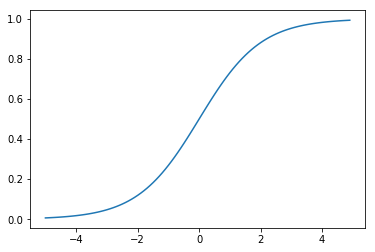
\includegraphics[scale=0.65]{sigmoidplot}
		\centering
	\end{figure}

	\textbf{Why is logistic function so important?}
	Because it can take any real input $x, (x \in R)$, whereas the output always takes values between 0 and 1, and hence is interpretable as probability.
	

	
\end{document}